\documentclass{beamer}

\usetheme{Darmstadt}
\usecolortheme{crane}

\usepackage[T1]{fontenc}
\usepackage{eurosym}
\usepackage{lmodern}
\usepackage[utf8]{inputenc}
\usepackage[french]{babel}
\usepackage{listings}


\title{My Oak}
\subtitle{Une application Android pour OwnCloud}
\author{Abdoulaye Dramé, Thibaud Destouches \& Marceau Lacroix}
\institute{ISTIC}
\date{}
\AtBeginSection[]
{
  \begin{frame}<beamer>{Plan}
    \tableofcontents[currentsection]
  \end{frame}
}
\begin{document}
\begin{frame}
\titlepage
\end{frame}

\begin{frame}
\frametitle{Plan}
\tableofcontents
\end{frame}




\section{Introduction}

	\begin{frame}{OwnCloud, c'est quoi ça?}
	\begin{itemize}
	\item Une application de synchronisation de:
		\begin{itemize}
		\item Fichiers
		\item Contacts
		\item Calendriers
		\end{itemize}
	\item Similaire à dropbox, mais chez soi!
	\item Opensource
	\end{itemize}
	\end{frame}

	\begin{frame}{Pourquoi faire une application android?}
	\begin{itemize}
	\item Acceder à ses données de partout
	\pause
	\item Synchroniser les contacts "chez soi"
	\pause
	\item Application déjà existante de mauvaise qualité
	\end{itemize}
	\end{frame}


\section{Architecture}
\begin{frame}{Architecture}
	\hspace{2.5cm} 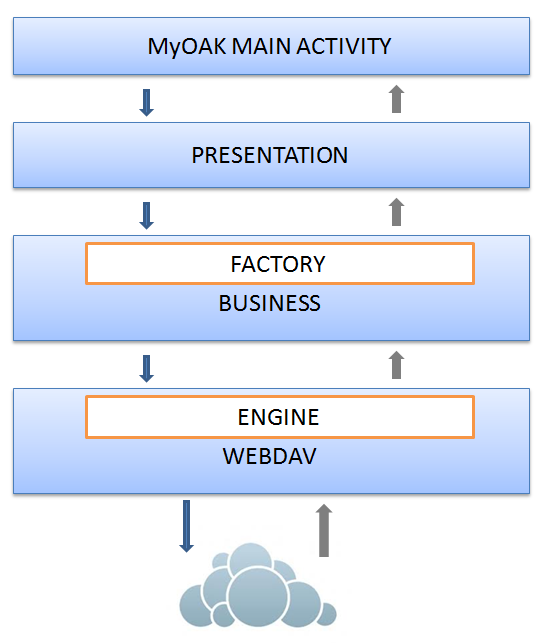
\includegraphics[scale=0.42]{img/Archi}
\end{frame}

\begin{frame}{WebDAV}
	\begin{itemize}
	\item \textbf{Web} \textbf{D}istributed \textbf{A}uthoring and \textbf{V}ersioning
	\item Extension du protocole HTTP
	\item But: Facilciter la gestion des fichiers avec des serveurs distants
		\begin{itemize}
		\item Récupérer
		\item Déposer
		\item Synchroniser
		\item Publier
		\item Accès concurrents
		\end{itemize}
	\end{itemize}
\end{frame}
		
\begin{frame}{Business}
	\begin{itemize}
		\item Couche métier
		\item Design pattern Composite
	\end{itemize}
	\hspace{3cm} 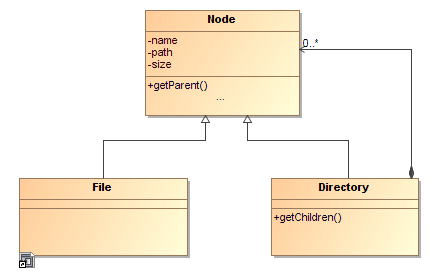
\includegraphics[scale=0.6]{img/designComposite}
\end{frame}		
		
\begin{frame}{Présentation}
	\begin{itemize}
		\item Séparation avec les modèles métiers
		\item Utilisation de la délégation
	\end{itemize}
	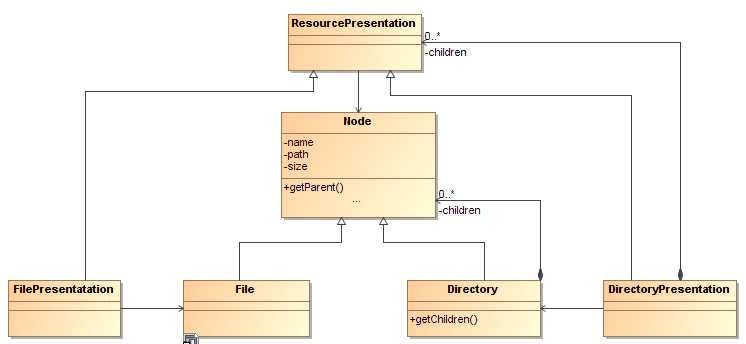
\includegraphics[scale=0.5]{img/presentation}
\end{frame}	

\begin{frame}{MyOAK Main Activity}
	\begin{itemize}
		\item Activité principale et unique de l’application
			\begin{itemize}
			\item Un fragment statique (Menu général)
			\item Un fragment dynamique
			\end{itemize}
		\item Un fragment pour chaque menu
		\item Chaque fragment ajoute ses options dans la barre d’action
	\end{itemize}
\end{frame}	




\section{Difficultés rencontrées}
\begin{frame}{Difficultés}
	\begin{itemize}
	\item Manque de temps
	\item API ownCloud obscure
	\item Les salles de l'université qui ferment à 22h
	\end{itemize}
	\end{frame}


\section{Démonstration}

\section{Conclusion}
	\begin{frame}{Conclusion}
	\begin{itemize}
	\item Ce qui marche:
		\begin{itemize}
		\item navigation dans les repertoires de fichiers
		\item Suppression de fichiers et de dossiers
		\item Ouverture de fichiers
		\item Ajout de dossier 
		\end{itemize}
	\pause
	\item Ce qui n'est pas encore implémenté:
		\begin{itemize}
		\item Ajout de fichiers
		\item Synchronisation de contacts
		\item Gestion des calendriers
		\item Streaming de musique
		\end{itemize}
	\end{itemize}
	\end{frame}


\end{document}
